\section{Præsentation af data}
\label{TestAfSkalaPraesentationAfData}
%
I følgende afsnit vil det indsamlede data blive præsenteret. Dette dækker over den gennemsnitlige besvarelse til hver af de 23 skalaer, kønsfordeling i forhold til den gennemsnitlige besvarelse, fordelingen af alder og højde samt hvor glade testpersonerne er for teknologi. 
%
\begin{figure}[H]
\centering
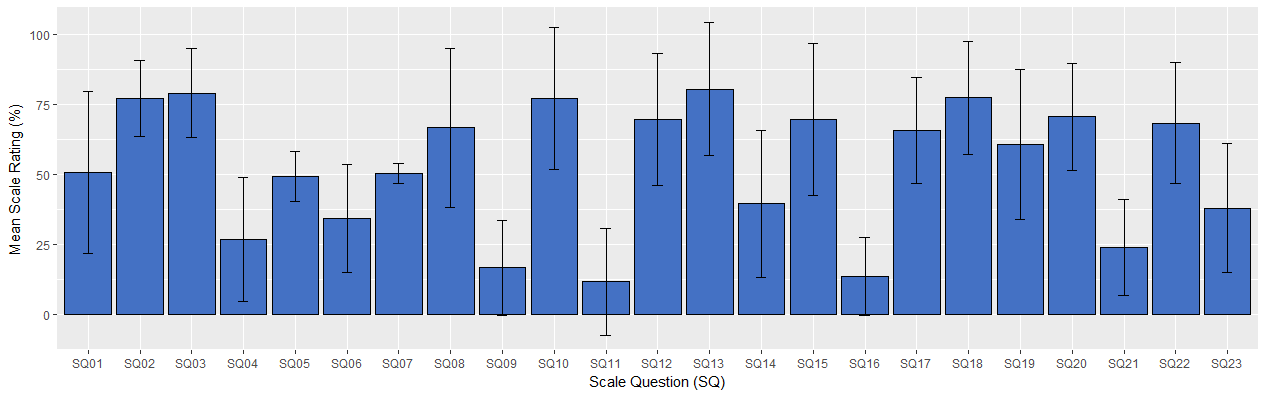
\includegraphics[width = \textwidth]{Figure/DatabehandlingSkalaer/DataPresentation/MeanBarplot} 
\caption{Søjlediagram over den gennemsnitlige besvarelse (\%) til hvert skala spørgsmål (SQ).}
\label{fig:BarPlotGennemsnit}
\end{figure}
\noindent
%
På \autoref{fig:BarPlotGennemsnit} fremgår den gennemsnitlige besvarelse for hver af de 23 skalaer, angivet med \textit{SQ} efterfulgt af nummer.

